\documentclass[a4paper]{article}

\usepackage[utf8]{inputenc}
\usepackage[T1]{fontenc}
%\usepackage{fontspec}
%\usepackage{xunicode}
\usepackage[francais]{babel}
\usepackage{color}
\usepackage[usenames,dvipsnames,svgnames,table]{xcolor}
\usepackage{lmodern}
\usepackage{lastpage}
\usepackage{graphicx}
\usepackage{fancyhdr}
\usepackage{geometry}
%\usepackage{layout}
%\usepackage{setspace}
%\usepackage{soul}
%\usepackage{ulem}
%\usepackage{eurosym}
%\usepackage{bookman}
%\usepackage{charter}
%\usepackage{newcent}
%\usepackage{mathpazo}
%\usepackage{mathptmx}
%\usepackage{url}
%\usepackage{verbatim}
%\usepackage{moreverb}
\usepackage{listings}
%\usepackage{wrapfig}
%\usepackage{colortbl}
%\usepackage{amsmath}
\usepackage{amssymb}
%\usepackage{mathrsfs}
%\usepackage{asmthm}
%\usepackage{makeidx}
\usepackage{tabularx}


\geometry{top=2.5cm, bottom=2cm, left=2cm, right=2cm}
\setcounter{tocdepth}{3}

%%%%%%%  VARIABLES     %%%%%%%%%%%%%%%%%%%%%%%%%%%%%%%%%%%%%
\newcommand{\docsauthor}{GARANDEL Adrien \& RUCHAUD Alexis}
\newcommand{\docstitle}{Labyrinth RPG}
%%%%%%%%%%%%%%%%%%%%%%%%%%%%%%%%%%%%%%%%%%%%%%%%%%%%%%%%%%%%

%%%%%%%   MAKE TITLE   %%%%%%%%%%%%%%%%%%%%%%%%%%%%%%%%%%%%%
\author{\docsauthor}
\title{\docstitle}
\date{\today}
%%%%%%%%%%%%%%%%%%%%%%%%%%%%%%%%%%%%%%%%%%%%%%%%%%%%%%%%%%%%

%%%%%%  EN-TETE / PIED-PAGE %%%%%%%%%%%%%%%%%%%%%%%%%%%%%%%%
\pagestyle{fancy}
\fancyhead{}
\fancyfoot{}
\lhead{\docsauthor}
\rhead{\docstitle}
\rfoot{\thepage/\pageref{LastPage}}
\lfoot{} %$\backslash\_0< Koin !$}
\renewcommand{\footrulewidth}{0.5pt}
\renewcommand{\headrulewidth}{0.5pt}
%%%%%%%%%%%%%%%%%%%%%%%%%%%%%%%%%%%%%%%%%%%%%%%%%%%%%%%%%%%%

%%%%%%  SETTING COLOR %%%%%%%%%%%%%%%%%%%%%%%%%%%%%%%%%%%%%%
\definecolor{key}{rgb}{0.6,0,0.6}
\definecolor{bck}{rgb}{0.92,0.92,0.92}
\definecolor{comment}{rgb}{0.5,0.5,0.5}
\definecolor{string}{rgb}{0,0.5,0}
\definecolor{number}{rgb}{0,0.5,0.5}
%%%%%%%%%%%%%%%%%%%%%%%%%%%%%%%%%%%%%%%%%%%%%%%%%%%%%%%%%%%%

%%%%%% SETTING %%%%%%%%%%%%%%%%%%%%%%%%%%%%%%%%%%%%%%%%%%%%%
\lstset{
language=C++,
basicstyle=\fontfamily{lmtt} \small,
numbers=left,
numbersep=7pt,
numberstyle=\small,
showspaces=false,
showtabs=false,
tabsize=4,
xleftmargin=20pt,
xrightmargin=20pt,
morekeywords={},
%backgroundcolor=\color{bck},
commentstyle=\color{comment},
keywordstyle=\color{string},
breaklines=true
}

\renewcommand{\FrenchLabelItem}{\space\textbullet}

\setlength{\parskip}{1ex plus .8ex minus .8ex}
\setlength{\parindent}{.8em}

%%%%%%%%%%%%%%%%%%%%%%%%%%%%%%%%%%%%%%%%%%%%%%%%%%%%%%%%%%%%

\begin{document}

	\maketitle{}
	\thispagestyle{empty}
	\newpage
	\tableofcontents{}
	\newpage
	\section{Introduction}

Le but de ce projet est d’implémenter un programme C++ en y incluant 4 design pattern.
Nous avons choisi pour ce projet de créer un jeu sous forme de labyrinthe en 2D. L'objectif du joueur sera
de trouver la sortie du labyrinthe en affrontant les monstres qui s'y trouvent. Pour cela il trouvera des équipements soit
en tuant ces monstres soit en ouvrant des coffres à trésor éparpillés dans le labyrinthe.
Pour ce faire nous avons utilisés le pattern State , Strategy , Absract Factory et enfin le pattern Decorator. Nous détaillerons plus tard
le fonctionnement de ces patterns au sein de notre programme avec l'appui d'un diagramme UML pour chaque pattern.
Premièrement nous allons vous donner les instructions de compilations, puis nous verrons le fonctionnement général du programme.
Deuxièmement nous regarderons en détail l'utilisation des design pattern puis des autres classes du programme
Enfin , nous finirons par la conclusion avec nos ressenti sur le projet , les difficultés rencontrées ainsi que les améliorations futures
que nous pourrions apporter au programme.


	\section{Fonctionnement général}

    \subsection{Compilation et exécution}
        
 La compilation et l’exécution du programme sont extrêmement simple. Il suffit de ce rendre, avec le terminal Linux, dans le dossier contenant
 les sources du programmes et d'entrer "make all" .
 Une fois la compilation des classes terminée il faudra pour exécuter le programme simplement taper "./laby".
 
    \subsection{Carte et déplacements}
    
 Au lancement du programme , une aide apparaît indiquant au joueur comment se déplacer dans le labyrinthe : "z" pour aller vers le haut/nord , "s" pour aller vers 
 le bas/sud , "q" pour aller à
 gauche/ l' ouest , "d" pour aller à droite/l'est et enfin "h" pour ré-afficher l'aide.
 Au départ il n'y a qu'une case visible pour le joueur et c'est lors de ses déplacements qu'il découvrira peu a peu le labyrinthe.
 A chaque fois que le personnage avance d'une case le labyrinthe est ré-afficher entièrement pour qu'il puisse suivre sa position aisément. Ses statistiques et
 ses équipements sont eux aussi affiché à chaque déplacement afin que le joueur puisse garder un oeil sur ses statistiques, équipements et surtout point de vie qui, à chaque
 deplacement seront un petit peu régénéré
 Le labyrinthe est composé de salles vides et de salles contenant soit un monstre soit un coffre et enfin la case de sortie.
 Les cases non vides sont nommés par un label sur le labyrinthe (Me pour la position du personnage,Mn pour Monstre , Tr pour Trésor,St pour le point de départ et Ed pour la sortie).
 Enfin, lors d'arriver du personnage sur la case sortie, celui-ci devra combattre (et vaincre) un monstre de niveau 10 afin de terminer la partie.
 
   \subsection{Combats}
   
  Lorsque le joueur arrive sur une case Monstre, un message lui indique le niveau du monstre ( Niveau de 1 à 10 ) et lui demande si il souhaite le
  combattre ou non. Si le joueur choisit de ne pas combattre le monstre il retourne automatiquement à sa position précédente et peu continuer son exploration.
  Dans le cas contraire, si le joueur choisit de se battre, le combat contre le monstre débute. Le combat est automatique. A tour de rôle le monstre
  et le joueur vont s'échanger des coups jusqu'a ce que l'un des deux meurs. Si le monstre bat le joueur la partie est terminée , si c'est le joueur qui 
  bat le monstre un nouveau message apparaît pour lui proposer d'ouvrir un coffre qui contiendra du butin en fonction du niveau du monstre (avec quand même toujours une composante aléatoire).
  La case de fin étant toujours accompagnée d'un monstre de niveau maximum, il est vivement recommandé au joueur de tenter d'affronter le plus de monstre avant de s'y confronter
  afin de récupérer le maximum de butin.
 
	\newpage
    \section{Design Pattern}
 
      \subsection{Pattern State}
      \subsection{Pattern Strategy}
      \newpage
      \subsection{Pattern Abstract Factory}
	  \begin{figure}[h]
		\centering
			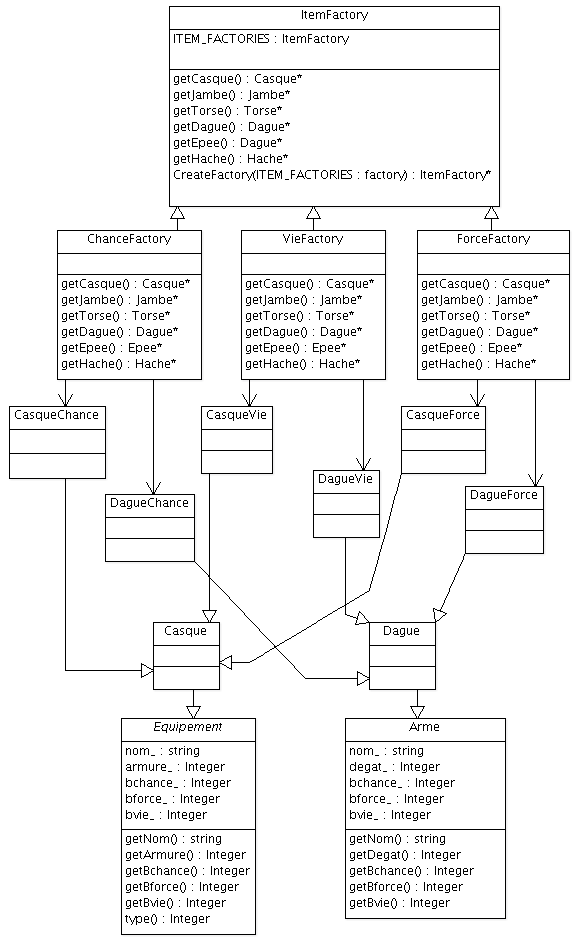
\includegraphics[width=11.5cm]{./Factory_UML.png}
		\caption{UML : Pattern Abstract Factory}
		\label{fig:Factory_UML}
	  \end{figure}
	\newpage
Le pattern abstract factory utilisé ici permet la création des équipements et des armes pour le personnage.
Il est composé d'une classe abstraite ItemFactory , de 3 factory concrètes qui en découlent : ChanceFactory , ForceFactory et VieFactory
Ces factory permettent de créer différents types d'objets.6 classe abstraite d'objet : Dague, Epee, Hache, Casque, Jambe et Torse.
Ces 6 classes abstraites possèdent chacunes 3 classes filles qui sont les objets concrets (Ex : EpeeVie , CasqueChance , JambeForce etc...).
Le fonctionnement de ce pattern est simple : La classe ItemFactory créer lors de l'appel de sa méthode une factory concrète en fonction du type
passé en paramètre (CHANCEF,FORCEF,VIEF). Ensuite cette factory concrète va créer des objets en fonction de la méthode appelée.
Par exemple une factory de type chance (ChanceFactory) créera un item de type HacheChance si la méthode getHache() est appelée.

L'utilisation de ce pattern pour gérer les équipements et armes permet une bonne encapsulation des classes lors de leur création. Cela facilite
aussi grandement la création des équipements et des armes en les faisant créer par la factory.


Sur le diagramme UML (fig \ref{fig:Factory_UML}), nous n'avons pas mis toutes les classes abstraites et concrètes des Armes et Équipements car cela prenait beaucoup de place.
Il y a donc Jambe, JambeChance , JambeForce, JambeVie, Torse , TorseChance, TorseForce, TorseVie, Epee, EpeeChance, EpeeForce, EpeeVie , Hache,
HacheChance , HacheForce et HacheVie qui manque sur la diagramme, en effet , elles sont très proche de Dague, Casque et leurs classes filles
déjà présentes.

		

      \subsection{Pattern Decorator}
      \begin{figure}[h]
			\centering
				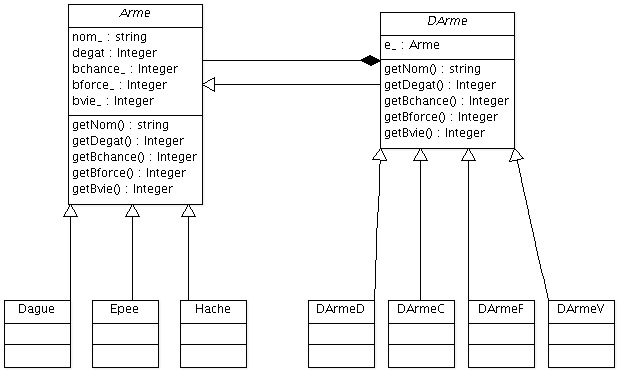
\includegraphics[width=15cm]{./Decorator_UML.png}
			\caption{\label{fig:Decorator_UML}UML : Pattern Decorator}
			
		\end{figure}
Ce programme implémente deux Decorators différent. Un pour les Armes et un pour les Équipements. Ici le diagramme UML est celui du decorator
d'arme néanmoins celui des équipements est quasiment identique à celui-ci.

Le pattern decorator utilisé ici permet de décorer les objets précédemment créer par les factory. Ainsi un objet "Casque de Vie" donnant +X à la vie
du personnage pourra être décoré en "Casque de Vie+1" donnant +X+Y à la vie du personnage, ou bien en "Casque de Vie de Force" donnant +X à la vie 
et +Y à la force du personnage. Tout cela selon les décorations appliquées à l'objet.
Ce pattern est composé d'une classe DArme qui hérite de la classe abstraite Arme et qui possède un attribut Arme. Grâce à celui-ci des bonus sont ajoutés à l'objet lors de sa décoration et son nom change. Pour le nom,on ajoute respectivement "de Force", "de Vie","de Chance", "de Degat" ou "d'Armure" si l'on décore avec de la force, de la vie, de la chance, du dégât ou de l'armure. Ensuite si le nom de l'objet est déjà composé d'une de ces chaînes et que l'on le décore a nouveau l'objet qui devrait devenir par exemple :
"Casque de Force de Force", il deviendra "Casque de Force+1 " puis "Casque de Force+2" selon le nombre de fois ou il est décoré. Ses bonus serons aussi modifiés.

L'utilisation de ce pattern nous permet de créer un très grand nombre d'objet différent sans avoir à créer des centaines de classes. Ainsi pas besoin d'avoir une classe spécifique pour créer un objet du genre "Epee Puissante+2 de Force+9 de Vie+2 de Chance+4"

 
 \section{Conclusion}
 
    En conclusion, ce projet nous auras permis de voir l'utilité des Design Pattern dans un contexte "réel" et de remarquer que si ils sont bien utilisés ils permettent de gagner énormément de temps. De plus le code est largement simplifié par leur utilisation et un problème que l'on aurais pus résoudre avec de très nombreuses classes se résous finalement en très peu de place.
De plus, le fait que le projet soit libre, pas de consigne imposée(patterns mis à part), nous a permis de nous investir plus facilement dans l'implémentation du programme.
En effet, un sujet imposé et beaucoup moins motivant, celui-ci ne laissant que très peu de place à l'imagination.
Par contre, il est beaucoup plus difficile de commencer un projet lorsqu'il est libre. Car n'ayant pas de fil directeur il est parfois un peu dur de savoir ce qu'il faut
commencer à implementer et ce qui peut attendre. Surtout lorsque l'on à pas encore une idée fixe sur le programme.

Pour la suite du programme et pour l'améliorer, il y a plusieurs choses que nous pourrions faire.
Tout d'abord, l'implémentation d'une interface graphique pour le labyrinthe et de sprite pour le joueur et les monstres pourraient rendre le jeu beaucoup plus immersif
que l'aspect simpliste de la console. Ensuite la création d'un inventaire pour le personnage serait enviseagable et permettrait l'apparition de consommable tel des potions
qui pourrait renforcer le personnage pour un certain temps ou nombre de combats.
Les combats pourraient être aussi améliorer afin d'impliquer le joueur qui, ici, doit juste attendre de voir si il gagne ou si il perd.
Enfin, plusieurs niveau de labyrinthe et des monstres de plus en plus fort permettrait d'améliorer grandement la durée d'une partie.

Pour finir même si l'implémentation du jeu c'est plutôt bien déroulé, quelques problèmes nous ont quelques fois ralentis. Par exemple, au niveau du pattern Decorator
où lorsqu'un objet était décoré 10 fois ou plus, il devenait très long de recréer le nom de cet objet. Ce problème venait du fait que la méthode qui reconstruit le nom
des objets s'appelait récursivement et amenait à des temps d'exécution extrèmement long. Pour régler ce problème nous avons dû modifier directement le nom de l'objet de
base plutôt que de modifier la chaîne de caractère lors de l'appel du nom de l'objet.

\begin{figure}[h]
			\centering
				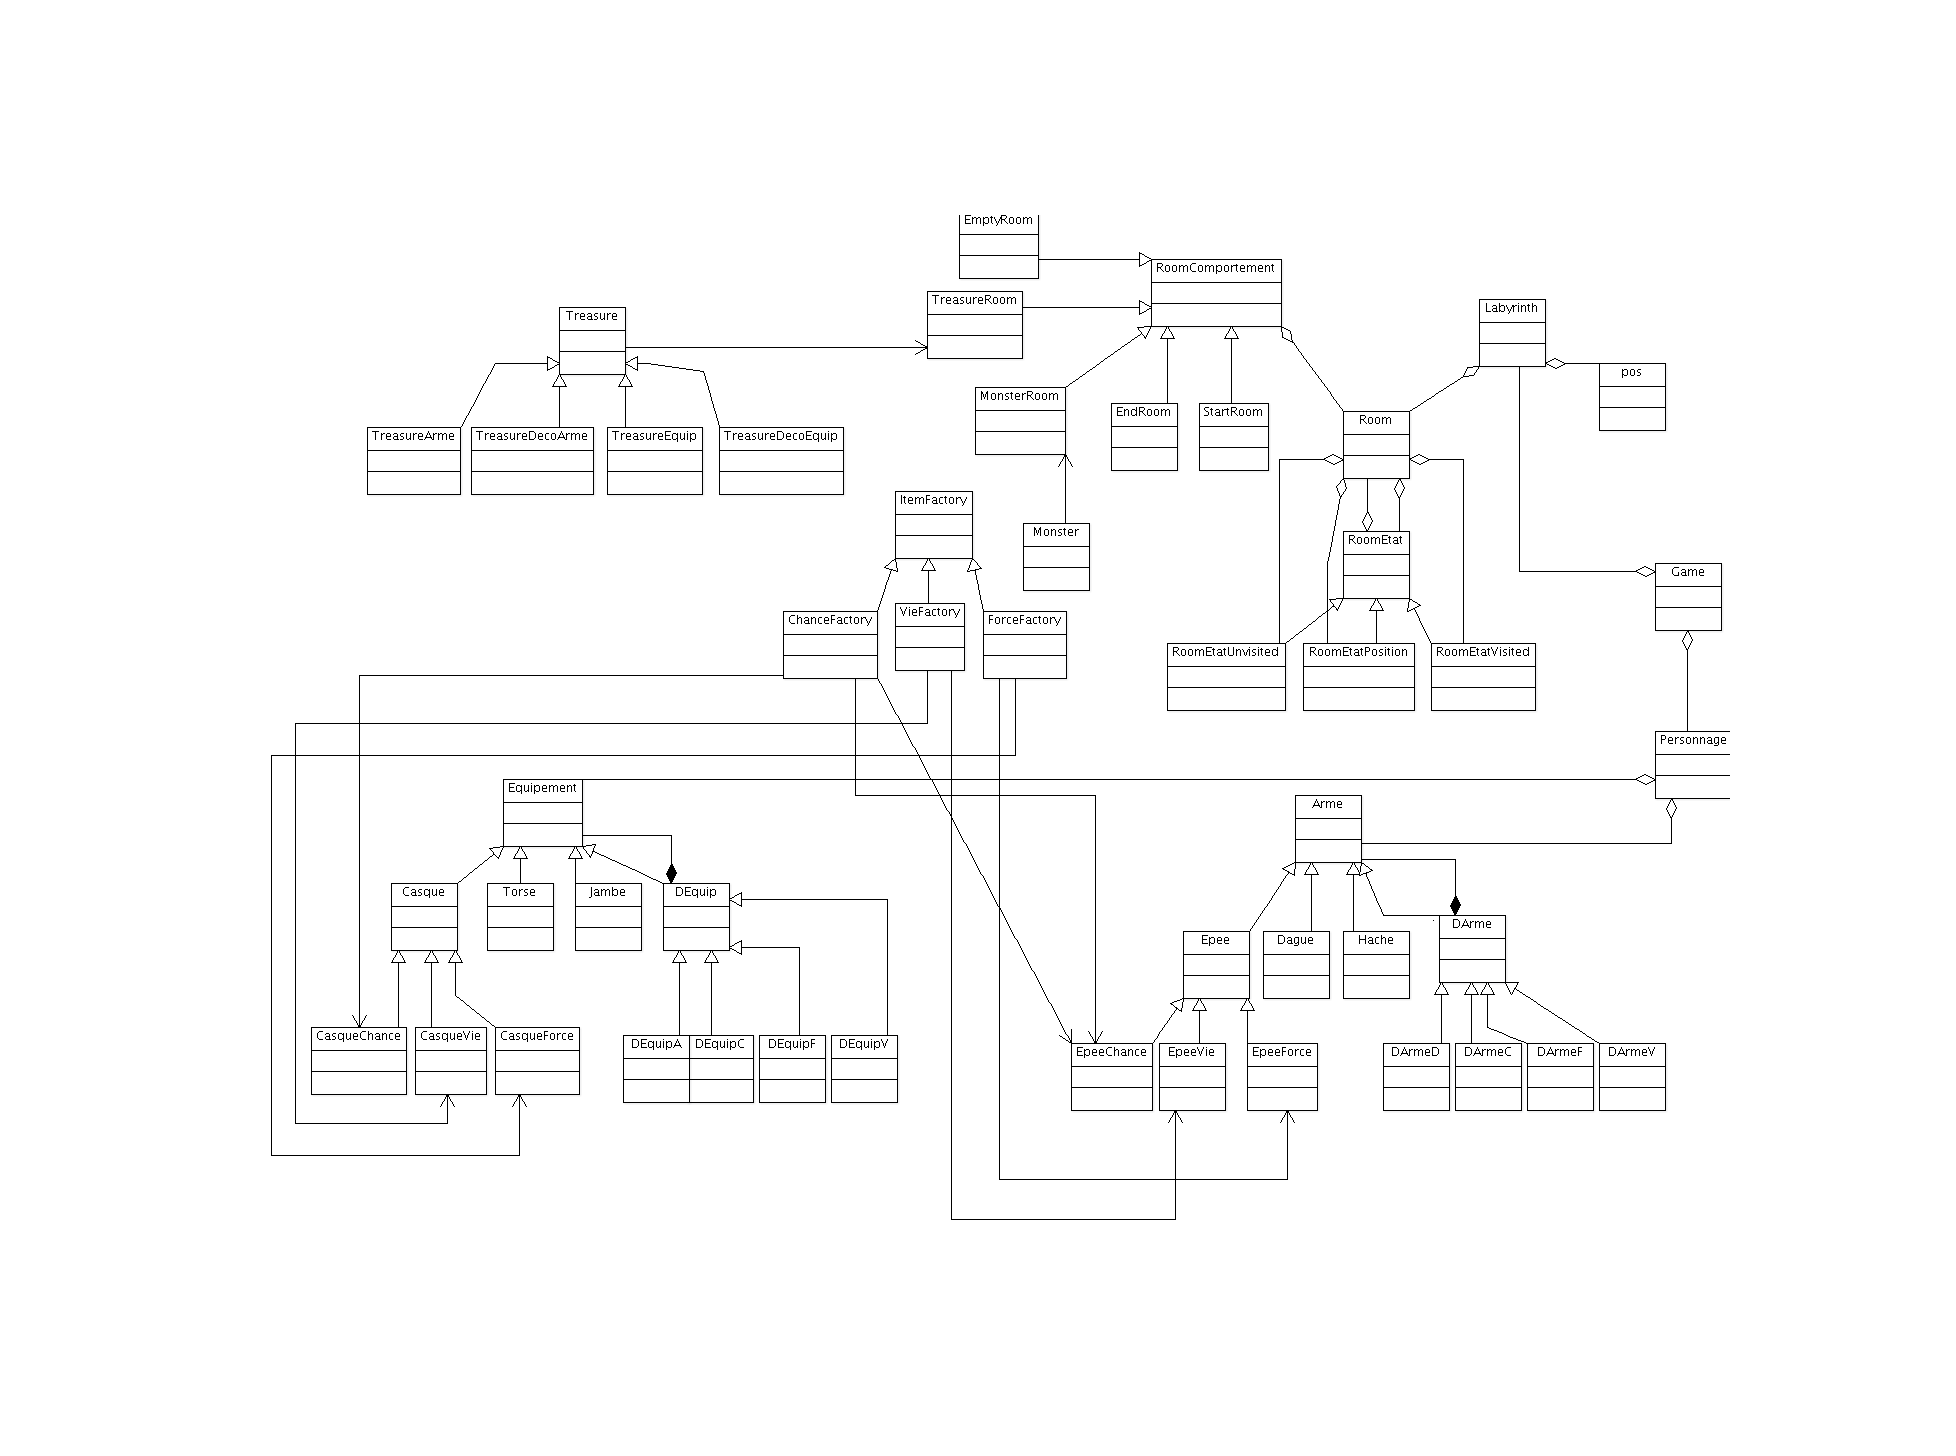
\includegraphics[angle=90,width=20cm]{./diagClasse.png}
			\caption{\label{fig:Diag}Diagramme De Classe}
			
		\end{figure}
\end{document}

